\documentclass[tikz]{standalone}
\usepackage{eulervm}
\usepackage[osf,sc]{mathpazo}
\usepackage{inconsolata}
\usetikzlibrary{calc}
\usepackage{graphicx}
\newcommand{\rdf}{{
\includegraphics[scale=0.02]{rdf.png}}}
\newcommand{\drdf}[1]{%
	\node[above=10cm of #1] (rdf#1) {\qquad\qquad\rdf}; %
	\draw[->,line cap=round,rounded corners,draw=blue,double=green,double distance=1.6pt,->] (#1.east)  -- node [right,midway] {$\color{blue}\alpha$} ($(rdf#1.south east)!.5!(rdf#1.south)$);
}
\newcommand{\wrdf}[1]{%
	\node[right=.2mm of #1] (rdf#1) {\rdf}; %∑
}
\usetikzlibrary{chains,backgrounds,fit,calc}
\begin{document}
\begin{tikzpicture}[
  >=latex, thick,
  node distance=1cm and 2cm,
  my edge/.style={->}, my edge'/.style={<-},
  box/.style={
    shape=rectangle, draw, fill, font=\strut,
    rounded corners},
  wh box/.style={box, fill=white, Minimum Height=all,inner sep=0pt, text width=24mm,align=center},
  bl box/.style={box, text=white, align=center, text width=1.8cm, Minimum Height=all},
  gr box/.style={box, thick, inner sep=+.5cm, draw=gray, fill=gray!25}
]

%% Level line
\draw[dashed] (-3.5,3.2) -- (24,3.2);


%% Global Data
\draw[fill=black,opacity=.2,very thick,draw=black,text=white] (24.4,-10) rectangle (25.4,18);
\node at ($(24.4,-10)!.5!(25.4,18)$) {\rotatebox{90}{\huge{\texttt{Global Data}}}};

%% Local Data
\draw[fill=black,opacity=.2,very thick,draw=black,text=white] (-3.5,18) rectangle (11,19);
\node[text=white] at ($(-3.5,18)!.5!(11,19)$) {{\huge{{Local Data}}}};

%% Data Integration Framework
\draw[fill=black,opacity=.2,very thick,draw=black,text=white] (11,18) rectangle (25.4,19);
\node[text=white] at ($(11,18)!.5!(25.4,19)$) {{\huge{{Data Integration Framework}}}};

%%%%%%%%%%%%%%%%%%%
%% LOCAL SOURCES %%
%%%%%%%%%%%%%%%%%%%

%% Please note that, in the meantime, I set up the meta level by drawing the \alpha edges alongside with the ontology extraction



%%%\node (PDF) {
\includegraphics{pdf.pdf}};
%%%%\drdf{PDF};
%%%
%%%\node[right=of PDF] (DOC) {
\includegraphics{doc.pdf}};
%%%%\drdf{DOC};
%%%
%%%\node[right=of DOC] (TXT) {
\includegraphics{txt.pdf}};
%%%%\drdf{TXT};

%\node[below left=4cm of PDF] (a) {};
%\node[below =of PDF] (b) {};

\node 
%at ($(a)!.5!(b)$) 
(HTML) {
\includegraphics{html.pdf}};
\drdf{HTML};

\node[right=of HTML] (XML) {
\includegraphics{xml.pdf}};
\drdf{XML};

\node[right=of XML] (JSON) {
\includegraphics{json.pdf}};
\drdf{JSON};

\node[right=of JSON] (GDB) {
\includegraphics{graph.pdf}};
\drdf{GDB};


\node[below =2cm of JSON] (a) {};
\node[below =2cm of XML] (b) {};

%% STRUCTURED DOCUMENTS

\node at ($(a)!.2!(b)$) (SQL) {
\includegraphics{sql.pdf}};
\wrdf{SQL};
\node[above=10cm of SQL] (rdf2SQL) {\qquad\qquad\rdf};
\draw[->,draw=red] (rdfSQL) -- node[above,sloped,very near end,text=red] {same as} ($(rdf2SQL.south east)!.5!(rdf2SQL.south)$);
\draw[<-] (SQL.south east)  -| node [below,near start,align=center] {schema+\\constraints} (rdfSQL.south);
\node[right=of SQL] (CSV) {
\includegraphics{csv.pdf}};
\drdf{CSV};


\node[below=2cm of CSV] (TXT) {
\includegraphics{txt.pdf}};
%\drdf{TXT};
\node[left=of TXT] (DOC) {
\includegraphics{doc.pdf}};
%\drdf{DOC};
\node[left=of DOC] (PDF) {
\includegraphics{pdf.pdf}};
%\drdf{PDF};

\node[draw=black,fit = (PDF) (DOC) (TXT),label=above:{\textbf{Unstructured Documents}},rounded corners] (UD) {};

\node[draw=black,fit = (rdfHTML) (rdfXML) (rdfJSON) (rdfGDB) (rdfCSV),rounded corners,minimum height=2cm,label=above:{Local Data Ontologies}] (SMDO) {};

\node[draw=black,fit = (CSV) (SQL), label=above:{Structured Documents},rounded corners] (SD) {};

%
\node[draw=black,fit = (HTML) (XML) (JSON) (GDB), label=above:{\textbf{Semi-structured Documents}},rounded corners] (SMD) {};

%% ONTOLOGY ALIGNMENT



\node[right = 4cm of rdfGDB,label=below:{Ontology Aligner}] (A) {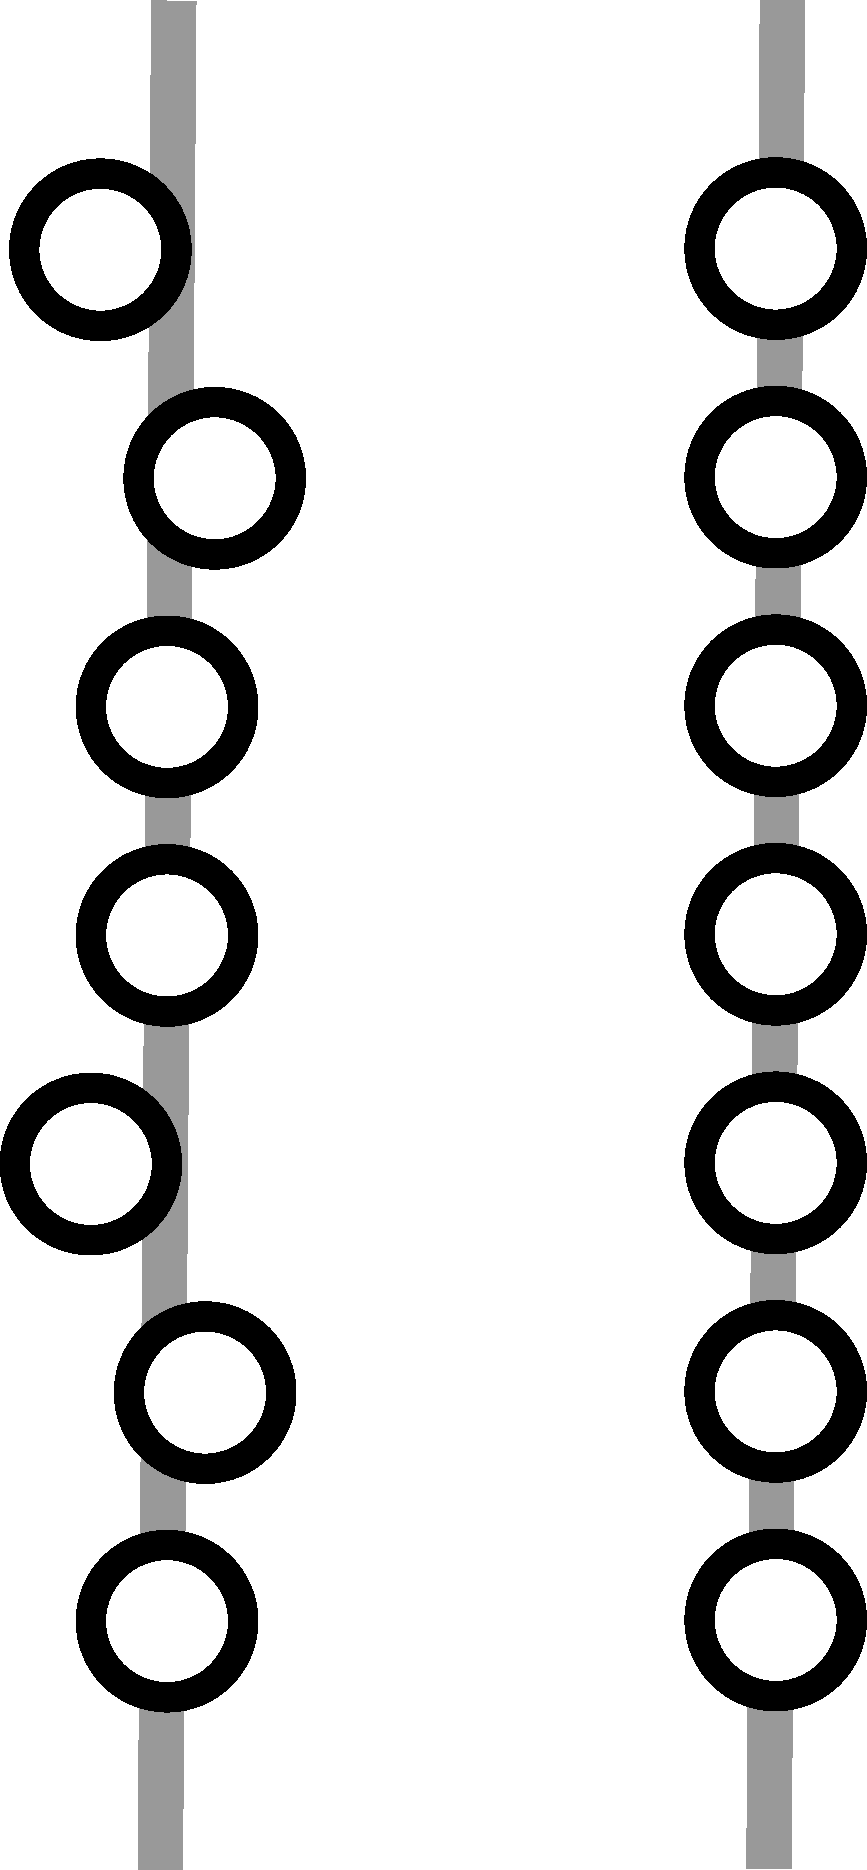
\includegraphics[scale=0.2]{align.pdf}};

\node[above left=1cm of A] (babelnet) {
\includegraphics[scale=0.2]{babelnet.png}};
\node[above=1cm of A] (icd10) {
\includegraphics[scale=0.3]{icd10.png}};
\node[above right=1cm of A] (mesh) {
\includegraphics[scale=0.13]{meshLogo.png}};
\draw[<->,color=green] (babelnet) -- (A);
\draw[<->,color=green] (icd10) -- (A);
\draw[<->,color=green] (mesh) -- (A);

\node at ($(SMDO.south east)!(A.west)!(SMDO.north east)$) (pt00) {};
\node at ($(pt00)+(1,0)$) (pt0d) {};
\draw[->,line width=3pt,blue] (pt00) -- node[above,midway] {\large{$\{L_1,\dots,L_9\}$}} (A);

\node[label=south:{Integrated Data}] at ($(SD)+(13,0)$) (V) {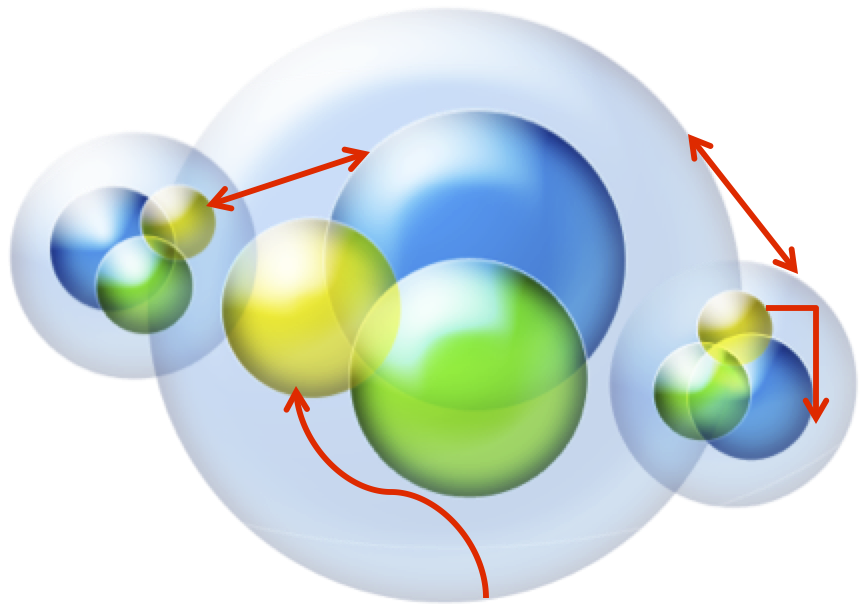
\includegraphics[scale=0.4]{nested.png}};


\node[label=below:{Hub Ontology},fill=yellow] at ($(pt00)!(V.north)!(pt0d)$) (H) {
\includegraphics[scale=0.7]{ontology.pdf}};

\node[right = 1cm of H] (qen) {};
\draw[->,line width=3pt,blue] ($(qen)+(3,0)$) -- node[above,midway,fill=yellow] {\large{query ($q$)}} (qen);

\draw[->,line width=3pt,blue] (H) -- node[above,midway] {\large{$H$}} (A);

\draw[->,line cap=round,rounded corners,draw=blue,double=green,double distance=1.6pt,->] ($(V.north west)!(H.south)!(V.north east)$)  -- node [right,near start] {$\color{blue}\alpha$} ($(H.south)-(0,1)$);
\draw[->] ($(A.south)-(0,1)$) |- node [near start,sloped,above] {integration} node [near start,sloped,below] (LAVGAV) {(LAV/GAV)} (V);

\node at ($(SMDO.east)-(0,1)$) (L) {};
\draw[->] ($(SMDO.east)!(LAVGAV)!(L)$) -- node [above,midway] {$\{D_1,\dots,D_9\}$} (LAVGAV);

\node at ($(qen)-(0,1)$) (qenq) {};
\node at ($(qen)!(V.east)!(qenq)$) (ven) {};
\draw[<-,line width=3pt,blue] ($(ven)+(3,0)$) -- node[above,midway] {\large{result}} (ven);

\end{tikzpicture}
\end{document}
